%==============================================================================
%  Paper 4 - Federated Cross-Dataset NIDS via Semantic Feature Alignment
%  Target venue: Journal of ICT Research and Applications (JICTRA), ITB (Scopus Q4)
%  Format disetarakan dgn pedoman JICTRA: TNR 11pt, abstrak 100-200 kata,
%  5-10 keyword, maks 20 halaman, gaya referensi IEEE (sesuai saran reviewer).
%  Catatan: naskah LaTeX; konversi ke template Word JICTRA pada tahap submit.
%==============================================================================
\documentclass[11pt,a4paper]{article}

\usepackage[utf8]{inputenc}
\usepackage[T1]{fontenc}
\usepackage{times}            % mendekati Times New Roman
\usepackage[english]{babel}
\usepackage{amsmath,amssymb}
\usepackage{geometry}
\geometry{margin=2.5cm}
\usepackage{booktabs}
\usepackage{array}
\usepackage{graphicx}
\graphicspath{{figure-fed/}{./}}
\usepackage{float}
\usepackage{enumitem}
\usepackage{tikz}
\usetikzlibrary{arrows.meta,positioning}
\usepackage[hidelinks]{hyperref}
\linespread{1.0}

% --- Longgarkan penempatan float agar tidak menumpuk di akhir dokumen ---
\renewcommand{\topfraction}{0.9}
\renewcommand{\bottomfraction}{0.9}
\renewcommand{\textfraction}{0.1}
\renewcommand{\floatpagefraction}{0.8}
\setcounter{topnumber}{3}
\setcounter{bottomnumber}{2}
\setcounter{totalnumber}{5}

\title{\textbf{When Does Cross-Dataset Federated Learning Work for Network
Intrusion Detection? A Controlled Study with Semantic Feature Alignment}}
\author{Hero Yudo Martono, Iwan Syarif, Ferry Astika Saputra\\
\small Politeknik Elektronika Negeri Surabaya (PENS), Surabaya, Indonesia\\
\small \texttt{hero@pens.ac.id, iwanarif@pens.ac.id, ferryas@pens.ac.id}}
\date{}

\begin{document}
\maketitle

%------------------------------------------------------------------
\begin{abstract}
\noindent
Federated learning (FL) lets organizations train a shared network intrusion
detection model without sharing raw traffic, but real deployments face
\emph{feature-schema heterogeneity}: clients extract features with different
tools, so their feature spaces differ. We study whether a
\emph{semantic feature alignment} --- mapping the features of different extraction
tools into a shared, semantically equivalent space --- can bridge this gap and
enable cross-dataset FL
between CSE-CIC-IDS2018 and UNSW-NB15. Using an identical lightweight model and
FedAvg across all settings, we run a controlled experiment that isolates the
effect of heterogeneity. On homogeneous partitions (one dataset split IID across
clients) FedAvg behaves normally, reaching Matthews correlation coefficient (MCC)
close to the centralized bound (0.563 and 0.674). A graded non-IID sweep locates a
sharp break point: the balanced dataset (UNSW) collapses near Dirichlet
\(\alpha\approx0.1\), while the benign-skewed dataset (CIC) stays stable. In the
true cross-dataset setting, naive FedAvg diverges (global MCC \(-0.026\)) and a
one-class autoencoder variant does not recover it. However, a
heterogeneity-aware strategy that shares a federated backbone while personalizing
the decision head (FedPer) raises the pooled test MCC (under personalized
evaluation) from \(-0.026\) to 0.731, close to the centralized upper bound. We conclude that semantic feature alignment is necessary
for interoperability but not sufficient under label-prior heterogeneity, that we
can quantify a measurable failure boundary, and that personalizing the federation
substantially reduces the performance gap under the studied cross-dataset setting.
\end{abstract}

\noindent\textbf{Keywords:} \emph{federated learning; network intrusion
detection; cross-dataset generalization; semantic feature alignment; non-IID;
data heterogeneity; FedAvg.}

\vspace{1em}

%==================================================================
\section{Introduction}
%==================================================================
Network Intrusion Detection Systems (NIDS) are a cornerstone of modern
cyber-defense, and machine learning (ML) has become the dominant approach for
building them because learned models generalize across attack variants better
than hand-written signatures. The vast majority of ML-based NIDS, however, are
trained in a \emph{centralized} manner: labeled traffic from many sources is
pooled on a single server, a detector is trained on the pool, and the detector is
then deployed. While convenient for research, this paradigm is increasingly
untenable in practice.

Two obstacles make centralized NIDS training problematic across organizations.
The first is \emph{privacy and regulation}. Network traffic contains sensitive
information --- internal addressing, service topology, user behavior --- and data
protection regulations as well as commercial confidentiality discourage, or
outright forbid, exporting raw traffic to a third party. The second, and the focus
of this paper, is \emph{feature-schema heterogeneity}: different organizations
instrument their networks with different flow-extraction tools (for example,
CICFlowMeter, Argus, Bro/Zeek, or NFStream), and each tool emits a different set
of features with different names, units, and semantics. Even when two
organizations observe comparable traffic, their feature vectors are not directly
comparable, so a model trained on one cannot be applied to the other.

Federated learning (FL) \cite{mcmahan} was designed to address the first obstacle:
clients train locally and exchange only model parameters, never raw data, so a
shared global model can be built without pooling. FL for intrusion detection has
consequently attracted significant attention \cite{ref-fl-survey,ref-fl-review}.
Yet standard FL --- in particular the canonical FedAvg algorithm --- implicitly
assumes that every client operates in an \emph{identical} feature space. That
assumption quietly reintroduces the second obstacle: if clients use different
extraction tools, their parameter vectors describe different input spaces and
cannot be averaged meaningfully. Most published FL-NIDS studies sidestep the issue
by taking a single public dataset and splitting it across simulated clients, so
the feature space is identical by construction and the distributions are close to
independent and identically distributed (IID). This is a convenient but
optimistic abstraction of the real cross-organization problem.

One way to bridge schema heterogeneity is \emph{semantic feature alignment}: a
dictionary that maps features from different extraction tools --- matched by
physical quantity, unit, and semantic meaning --- to a common feature space, so
that models expressed in that space become comparable. Such alignment has been used to improve \emph{centralized}
cross-dataset generalization. A natural question follows: can semantic feature
alignment also serve as an \emph{enabler} for federated learning across clients
that use different feature schemas, and how far does the resulting federated model
close the gap to a centralized one?

This paper answers that question with a \emph{controlled} empirical study rather
than a claim of superiority. Crucially, our setting departs from existing FL-NIDS
work in a specific way. Prior studies --- including state-of-the-art systems such
as Fed-ANIDS \cite{fedanids} --- partition a \emph{single} dataset across clients,
so all clients share one feature schema and a near-identical distribution. We
instead federate across \emph{two different-source datasets} (CIC and UNSW) whose
feature-extraction tools, feature schemas, and label priors all differ. This is
the harder, more realistic case that prior work avoids, and it is enabled only by
a validated semantic feature space. Our contributions are:
\begin{enumerate}[leftmargin=1.6em]
  \item \textbf{A new problem setting:} cross-dataset FL-NIDS across clients with
  \emph{different feature schemas}, bridged by a validated semantic feature
  alignment used as an interoperability enabler --- not a single dataset split, as
  in prior FL-NIDS work.
  \item \textbf{A systematic experimental framework} for identifying the
  \emph{failure boundary} of cross-dataset FL-NIDS under progressively increasing
  heterogeneity: by holding the model and aggregation fixed and varying only the
  degree of heterogeneity, the framework isolates the effect of heterogeneity and
  a homogeneous control confirms the pipeline is valid (near-centralized MCC). The
  contribution is thus not merely ``FedAvg fails'' but a methodology to measure
  \emph{when} and \emph{why} cross-dataset FL begins to fail.
  \item \textbf{A quantified break point:} a graded non-IID sweep that locates
  where FedAvg collapses and explains the asymmetry between a balanced and a
  benign-skewed dataset --- an analysis not reported for cross-dataset FL-NIDS.
  \item \textbf{A diagnosed negative result \emph{and} a working mitigation:} naive
  FedAvg diverges and a one-class autoencoder (the Fed-ANIDS paradigm) does not
  recover it, showing that semantic feature alignment is necessary but not
  sufficient under label-prior heterogeneity; yet a heterogeneity-aware strategy
  (FedPer, sharing a backbone while personalizing the head) restores
  near-centralized pooled test MCC, demonstrating that the failure boundary can be
  largely mitigated.
\end{enumerate}
To be explicit about scope: our novelty is in the \emph{problem framing, the
cross-schema federation via feature alignment, and the controlled
when-does-it-fail analysis},
not in a new aggregation algorithm. We reuse standard FedAvg/FedProx deliberately,
so that the observed behavior reflects the data heterogeneity we study rather than
a bespoke optimizer.

The remainder of the paper is organized as follows. Section~2 reviews related
work on FL-NIDS, data heterogeneity, feature alignment, and anomaly-based
detection, and positions our study. Section~3 describes the method: the semantic
feature mapping used as a public prior, the shared model and aggregation
algorithms, and the one-class variant. Section~4 details the controlled
experimental design, datasets, hyperparameters, and evaluation protocol.
Section~5 presents and discusses the five experimental stages in increasing order
of difficulty, from the homogeneous control to the cross-dataset case, the
one-class mitigation attempt, and the personalized-federation mitigation. Section~6 discusses threats to validity and
practical implications, and Section~7 concludes.

%==================================================================
\section{Related Work}
%==================================================================

\subsection{Federated learning for intrusion detection}
FL for intrusion detection has grown rapidly; recent surveys and taxonomies
catalog architectures, aggregation strategies, and open challenges
\cite{ref-fl-survey,ref-fl-review,wardana-survey,fedorchenko}. The dominant design
is a client--server topology in which a central aggregator maintains a global
model, broadcasts it, collects locally trained updates, and aggregates them with
FedAvg \cite{mcmahan}. Early collaborative-detection work established that
federated deep learning can match centralized detectors on shared benchmarks
\cite{popoola,agrawal}, and later systems extended FL-NIDS to edge, SDN, and
industrial-IoT settings \cite{chen-fedagru,doriguzzi-eff,mao-fedin}. DDoS-oriented
variants add clustering or adaptive client selection to the aggregator
\cite{lee-feddb,zainudin-fedddos,doriguzzi-flad}. Reported results are often
strong: with enough communication rounds, a federated detector approaches the
accuracy of a centralized one. However, the overwhelming
majority of these studies evaluate on a \emph{single} public dataset partitioned
across simulated clients, so the feature space is identical by construction and
the inter-client distributions are near-IID. Under those conditions FedAvg is
known to converge well, and the privacy benefit of FL comes almost for free.
Fed-ANIDS \cite{fedanids}, a representative state-of-the-art system, combines FL
with anomaly detection using autoencoders (simple, variational, and adversarial)
and reaches near-centralized F1 --- again on single-source data split across
clients. Our work keeps the same canonical machinery but changes the setting to
genuinely different-source datasets with different feature schemas.

\subsection{Data heterogeneity and non-IID federated learning}
It is well established that FedAvg degrades when client data is non-IID, because
local models drift toward their own distributions and their average no longer
represents a good global optimum \cite{ref-limits}. The degree of degradation
depends on the kind and severity of heterogeneity --- label skew, feature skew,
and quantity skew. Proximal methods such as FedProx \cite{fedprox} add a term that
penalizes divergence from the global model and improve stability, while
personalized, distillation-based, and clustered FL approaches
\cite{ref-personalized,benkaddour,ali-mist} abandon or soften a single global
model when clients are too different. Cross-domain alignment has also been applied
to vehicular and heterogeneous-IoT intrusion detection
\cite{khalid-fedcross,ks-ensemble}. The limits of FL under heterogeneity are now
explicitly studied \cite{ref-limits}, yet these methods mitigate but do not
eliminate the problem, and they are typically evaluated with synthetic non-IID
partitions of a single dataset rather than genuinely different datasets. Our
graded non-IID sweep follows this tradition but uses it as a diagnostic to locate
a break point, and then contrasts it against a real cross-dataset case.

\subsection{Feature alignment and cross-dataset generalization}
Cross-dataset generalization of NIDS is difficult precisely because feature
schemas and distributions differ between datasets. A line of work seeks a common
feature representation --- for example a standardized NetFlow feature set
\cite{sarhan} --- so
that models transfer across datasets. The \emph{semantic feature alignment} we use
belongs to this line: it builds a dictionary that maps features from different
extraction tools --- matched by physical quantity, unit, and semantic meaning ---
into a shared feature space, and such alignment has been shown to help
\emph{centralized} cross-dataset
generalization. Related efforts transfer knowledge across domains through
few-shot and meta-learning in a federated setting
\cite{hu-fewshot,mao-fecograph,yin-fedpkt,zhang-transfer,ceviz-fewshot}, and
cross-silo log-graph methods federate structurally different sources
\cite{xu-entente}. These address \emph{label} or \emph{sample} scarcity; the
present paper instead targets \emph{feature-schema} heterogeneity and asks whether
semantic alignment is also sufficient to enable \emph{federated} learning across
clients that use different extraction tools --- a question not previously examined.

\subsection{Anomaly-based detection}
An alternative to supervised classification is anomaly detection, in which a model
is trained only on normal traffic and attacks are flagged as deviations. This is
attractive when labeled attacks are scarce and when attack distributions differ
across sites. Autoencoder-based detectors measure reconstruction error, and
Fed-ANIDS \cite{fedanids} demonstrates their effectiveness in a homogeneous
federated setting; semi-supervised and generative federated variants pursue the
same idea with shrink autoencoders or GANs \cite{semisup-sae,bjorn-fgan,zeng-fga}.
We test whether the same paradigm helps in our heterogeneous cross-dataset
setting, where the label-prior mismatch that hurts supervised FedAvg is, in
principle, side-stepped.

\subsection{Adversarial robustness in federated NIDS}
A parallel concern is the robustness of federated detectors to adversarial or
poisoned updates. Robust aggregation, proximal defenses, and adversarial training
have been proposed to harden FL-NIDS \cite{ennaji-advrobust,chandu-hada,%
saha-krum,wang-robust}, and the broader adversarial-ML literature frames both
attacks and defenses on intrusion detectors \cite{debicha-advtrain,gadot}. These
works are complementary to ours: we study a benign failure mode (heterogeneity),
not an adversarial one, but the mitigation direction (personalized or robust
aggregation) overlaps.

\subsection{Positioning}

Table~\ref{tab:position} positions this work against representative FL-NIDS
studies along three axes that matter for our question: whether clients share one
feature schema, whether the data is single- or cross-source, and whether the
study isolates \emph{when} FL fails. To the best of our knowledge, we found no
prior FL-NIDS study that combines cross-schema federation (via a validated
semantic mapping) with a controlled break-point analysis across the
homogeneous-to-cross-dataset spectrum.
That combination is the gap this paper fills.

\begin{table}[htbp]
\centering\small
\caption{Positioning against representative FL-NIDS work.}
\label{tab:position}
\begin{tabular}{@{}lccc@{}}
\toprule
Study & Feature schema & Data source & Break-point analysis \\
\midrule
Fed-ANIDS \cite{fedanids}        & single & single-source split & no \\
FL-NIDS surveys \cite{ref-fl-survey,ref-fl-review} & single & single-source & no \\
Limits of FL \cite{ref-limits}   & single & single-source & partial \\
Personalized FL \cite{ref-personalized} & single & single-source & no \\
\textbf{This work}               & \textbf{different (aligned)} & \textbf{cross-dataset} & \textbf{yes (graded)} \\
\bottomrule
\end{tabular}
\end{table}

Our work therefore differs on all three axes: clients use \emph{different}
feature schemas reconciled by alignment, the federation is \emph{cross-dataset}, and we
frame the study around \emph{when} FL fails rather than asserting that it wins.

%==================================================================
\section{Method}
%==================================================================
\subsection{Semantic feature alignment (public prior)}
We define a semantic feature alignment between the two extraction tools: nine
semantically equivalent flow features that both CICFlowMeter (CIC) and Argus/Bro
(UNSW) can produce. Table~\ref{tab:align} lists the mapping. We constructed it by
matching column definitions across the two tools (e.g.\ ``Flow Duration'' $\equiv$
``dur'', ``Tot Fwd Pkts'' $\equiv$ ``spkts'') and validating, on each dataset
\emph{separately}, that the mapped features have comparable statistical meaning;
features without a semantically matching counterpart (for example tool-specific
TCP window encodings) are discarded rather than forced into correspondence. The
key property is that the mapping is a \emph{public prior} --- a dictionary of
column correspondences agreed \emph{before} any training, not learned from pooled
data. Each client applies the mapping to its own raw data locally to obtain the
nine common features; no raw data and no joint statistics are exchanged, which
preserves the privacy premise of FL. The alignment therefore functions as an
\emph{interlingua}: once each client expresses its traffic in the nine aligned
features, model weights live in a common space and can be averaged.

\begin{table}[htbp]
\centering\small
\caption{The nine aligned features: source columns, physical unit, and semantic
meaning (public prior). Each pair measures the same physical quantity under the
two tools; features without a semantically matching counterpart are excluded.}
\label{tab:align}
\begin{tabular}{@{}llll@{}}
\toprule
Aligned feature & CIC column (CICFlowMeter) & UNSW column (Argus/Bro) & Unit \\
\midrule
duration   & Flow Duration      & dur    & $\mu$s/s \\
fwd\_pkts  & Tot Fwd Pkts       & spkts  & count \\
bwd\_pkts  & Tot Bwd Pkts       & dpkts  & count \\
fwd\_bytes & TotLen Fwd Pkts    & sbytes & bytes \\
bwd\_bytes & TotLen Bwd Pkts    & dbytes & bytes \\
fwd\_mean  & Fwd Pkt Len Mean   & smean  & bytes \\
bwd\_mean  & Bwd Pkt Len Mean   & dmean  & bytes \\
src\_load  & Flow Byts/s        & sload  & bits/s \\
dst\_load  & Bwd Pkts/s         & dload  & bits/s \\
\bottomrule
\end{tabular}
\end{table}

\emph{Why these nine features.} The selection follows two rules that make it
reproducible. First, a feature pair is included only if both tools expose the same
physical quantity in the same unit (Table~\ref{tab:align}); counts, byte totals,
per-direction mean packet lengths, duration, and load rates satisfy this.
Second, pairs that are tool-specific or encoded differently are excluded rather
than forced into correspondence --- for example TCP window information is
continuous in CICFlowMeter but effectively categorical in the UNSW tool, so it is
dropped. The resulting nine features are the usable intersection of the two
schemas. For each pair we checked, on each dataset separately, that the feature is
present, numeric, and non-degenerate (non-constant), and we standardize per client
before training.

A consequence worth stating up front is that the aligned feature space is
optimized for \emph{alignment} --- it keeps only features whose semantics match
across tools --- and not necessarily for \emph{separability} of attacks. This
distinction becomes
important when we test anomaly detection (Section~\ref{sec:oc}), where we quantify
the separability of this space directly.

\subsection{Model and aggregation (held fixed across all settings)}
To make every setting comparable (apple-to-apple), we use one lightweight
multilayer perceptron (MLP) over the nine aligned features
(\(9\!\to\!128\!\to\!64\!\to\!1\), ReLU activations, sigmoid output) trained with
binary cross-entropy. The model is intentionally small: the goal is not to find
the best possible classifier but to study how federation behaves under
heterogeneity, so model capacity is held constant across every experiment.

Aggregation uses classic FedAvg \cite{mcmahan}. In each communication round
\(t\), the server broadcasts the global weights \(w^{(t)}\); each client \(k\)
trains locally for \(E\) epochs to obtain \(w_k^{(t)}\); the server then forms a
size-weighted average,
\begin{equation}
w^{(t+1)} = \sum_{k=1}^{K}\frac{n_k}{n}\,w_k^{(t)},\qquad n=\sum_{k=1}^{K} n_k,
\label{eq:fedavg}
\end{equation}
where \(n_k\) is the number of training samples at client \(k\). We also evaluate
FedProx \cite{fedprox}, which adds a proximal term to each client's local
objective to limit drift from the global model:
\begin{equation}
\min_{w}\;\mathcal{L}_k(w) + \frac{\mu}{2}\,\lVert w - w^{(t)}\rVert^2 ,
\label{eq:fedprox}
\end{equation}
with \(\mu \ge 0\) (\(\mu=0\) recovers FedAvg). Algorithm~\ref{alg:fed} summarizes
the loop. Per-client z-score normalization is computed locally from each client's
own training data, consistent with the privacy premise (no shared statistics).
Unless stated otherwise, hyperparameters are identical across all settings:
\(R=100\) rounds, \(E=5\) local epochs, learning rate \(3\times10^{-3}\), batch
size 256, seed 42 (five seeds for the significance test).

\begin{figure}[htbp]
\centering
\fbox{\begin{minipage}{0.92\columnwidth}\small
\textbf{Algorithm 1:} Federated training (FedAvg / FedProx)\\[2pt]
\textbf{Input:} clients \(1..K\) with local data; rounds \(R\); epochs \(E\);
learning rate \(\eta\); proximal \(\mu\)\\
\textbf{Output:} global weights \(w^{(R)}\)\\[2pt]
1.\ initialize global weights \(w^{(0)}\)\\
2.\ \textbf{for} \(t=0\) \textbf{to} \(R-1\) \textbf{do}\\
3.\ \quad broadcast \(w^{(t)}\) to all clients\\
4.\ \quad \textbf{for each} client \(k\) \textbf{in parallel do}\\
5.\ \qquad \(w_k \leftarrow\) train \(E\) epochs on local data from \(w^{(t)}\)
         (with proximal \(\mu\) if FedProx)\\
6.\ \quad \(w^{(t+1)} \leftarrow \sum_k (n_k/n)\, w_k\) \hfill (Eq.~\ref{eq:fedavg})\\
7.\ \textbf{return} \(w^{(R)}\)
\end{minipage}}
\caption{Federated training loop; only weights cross the network.}
\label{alg:fed}
\end{figure}

\subsection{One-class autoencoder variant}
\label{sec:ocmethod}
As a mitigation inspired by Fed-ANIDS \cite{fedanids}, we also study a one-class
autoencoder (AE). Each client trains an AE (\(9\!\to\!6\!\to\!3\!\to\!6\!\to\!9\),
Figure~\ref{fig:ae}) \emph{only on its normal traffic} by minimizing the mean
squared reconstruction error. Attacks are detected at inference as anomalies: a
sample \(x\) is flagged when its reconstruction error exceeds a threshold
\(\tau\),
\begin{equation}
s(x) = \lVert x - \mathrm{AE}(x)\rVert_2^2, \qquad \hat{y} = \mathbb{1}[\,s(x) > \tau\,],
\end{equation}
where \(\tau\) is calibrated as the 95th percentile of the reconstruction error on
normal training data. The federated AE averages weights with Eq.~\ref{eq:fedavg}
exactly as the supervised model. The rationale is that ``normal'' traffic may be
more similar across datasets than the supervised decision boundary, so the AE
weights might average more stably and side-step the label-prior mismatch.

\begin{figure}[htbp]
\centering
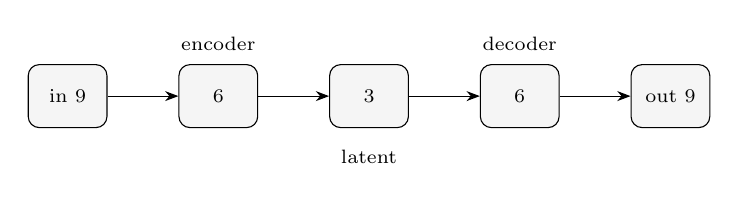
\begin{tikzpicture}[node distance=0.5cm and 0.9cm,font=\scriptsize,
  box/.style={draw,rounded corners,minimum height=0.8cm,minimum width=1.0cm,fill=black!4}]
  \node[box] (i) {in 9};
  \node[box,right=of i] (h1) {6};
  \node[box,right=of h1] (z) {3};
  \node[box,right=of z] (h2) {6};
  \node[box,right=of h2] (o) {out 9};
  \draw[-{Stealth}] (i)--(h1); \draw[-{Stealth}] (h1)--(z);
  \draw[-{Stealth}] (z)--(h2); \draw[-{Stealth}] (h2)--(o);
  \node[below=0.15cm of z,font=\scriptsize] {latent};
  \node[above=0.05cm of h1,font=\scriptsize] {encoder};
  \node[above=0.05cm of h2,font=\scriptsize] {decoder};
\end{tikzpicture}
\caption{One-class autoencoder: trained on normal traffic only; detection by
reconstruction error.}
\label{fig:ae}
\end{figure}

\subsection{Personalized federation (FedPer)}
\label{sec:fedper}
As a heterogeneity-aware alternative to a single global model, we use FedPer. The
same MLP is split into a \emph{shared backbone} (the two hidden layers,
\(9\!\to\!128\!\to\!64\)) and a \emph{personalized head} (the output layer,
\(64\!\to\!1\)); Figure~\ref{fig:fedper} illustrates the split. Only the backbone
is federated: in each round, every client trains the whole network locally, but
the server averages \emph{only} the backbone weights,
\begin{equation}
w_{\mathrm{backbone}}^{(t+1)} = \sum_{k=1}^{K}\frac{n_k}{n}\,
w_{\mathrm{backbone},k}^{(t)},
\label{eq:fedper}
\end{equation}
while each client keeps its own head \(w_{\mathrm{head},k}\) locally and never
sends it to the server. Intuitively, the shared backbone learns a common
representation of the aligned features, while each head adapts the decision
boundary to the client's own label prior --- directly countering the gradient
cancellation that sinks naive FedAvg (Section~\ref{sec:oc}). As a limiting case we
also report \emph{clustered FL}, in which each client keeps a \emph{full} private
model (no sharing); this coincides with local-only and serves only as an upper
reference for complete personalization, not as a federated method.

\begin{figure}[htbp]
\centering
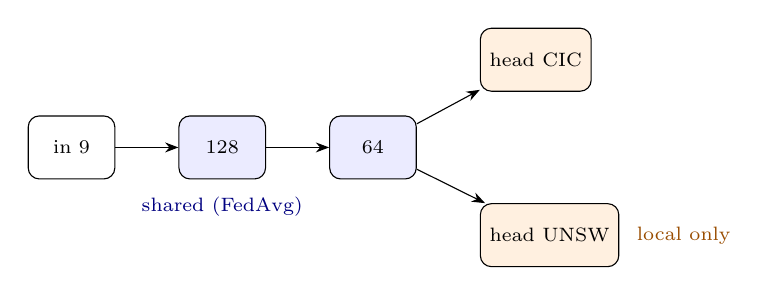
\begin{tikzpicture}[node distance=0.45cm and 0.8cm,font=\scriptsize,
  box/.style={draw,rounded corners,minimum height=0.8cm,minimum width=1.1cm},
  sh/.style={box,fill=blue!8}, hd/.style={box,fill=orange!12}]
  \node[box] (i) {in 9};
  \node[sh,right=of i] (h1) {128};
  \node[sh,right=of h1] (h2) {64};
  \node[hd,above right=0.3cm and 0.8cm of h2] (hc) {head CIC};
  \node[hd,below right=0.3cm and 0.8cm of h2] (hu) {head UNSW};
  \draw[-{Stealth}] (i)--(h1); \draw[-{Stealth}] (h1)--(h2);
  \draw[-{Stealth}] (h2)--(hc); \draw[-{Stealth}] (h2)--(hu);
  \node[below=0.1cm of h1,font=\scriptsize,text=blue!50!black] {shared (FedAvg)};
  \node[right=0.1cm of hu,font=\scriptsize,text=orange!60!black] {local only};
\end{tikzpicture}
\caption{FedPer: the backbone (blue) is federated via Eq.~\ref{eq:fedper}; each
client keeps a local, personalized head (orange) that is never shared.}
\label{fig:fedper}
\end{figure}

\paragraph{Personalized evaluation protocol.} Because FedPer has no single global
head, we state its evaluation explicitly. The shared backbone is identical across
clients. For CIC-test we use the CIC head, for UNSW-test the UNSW head, and for the
GLOBAL-test \emph{each sample is scored with the personalized head of its
originating client} (CIC samples through the CIC head, UNSW samples through the
UNSW head) on top of the common backbone. The GLOBAL-test number is therefore the
performance of the \emph{personalized federation} as a whole, not of a single
global classifier --- a distinction we make clear when interpreting the results.

\subsection{Metric}
We report the Matthews Correlation Coefficient (MCC) \cite{matthews} as the
primary metric,
because it is robust to the class imbalance common in NIDS traffic. MCC lies in
\([-1,1]\): \(1\) is perfect, \(0\) is random, and negative values indicate
anti-correlation (worse than random). We complement MCC with recall, precision,
F1, and balanced accuracy. We report per-client test sets (CIC-test, UNSW-test)
and a pooled GLOBAL-test, and we use five seeds \(\{13,42,101,202,303\}\) with a
paired significance test for the main comparison.

%==================================================================
\section{Experimental Design}
%==================================================================
Two datasets act as clients: CSE-CIC-IDS2018 (CIC) \cite{cicids} and UNSW-NB15
(UNSW) \cite{unsw}, both mapped to the nine aligned features. Table~\ref{tab:data} summarizes the per-client
statistics after a stratified subsample of CIC to balance client sizes.

This is a \emph{cross-silo} federated setting in the strict sense, not merely
distributed training. Each client holds its own private dataset that never leaves
the client: raw traffic and even per-client normalization statistics stay local,
and only model weights (the whole model for FedAvg, or the backbone for FedPer)
are exchanged with the server. The two clients deliberately differ in extraction
tool, feature schema, and label prior --- this heterogeneity is the independent
variable we study, not an artifact. Using exactly two silos is an intentional
design choice that \emph{isolates} cross-dataset heterogeneity from the confounding
effect of client count; the graded non-IID experiment (Section~\ref{sec:bridge})
separately varies the number of clients within a single dataset. The setting thus
mirrors two organizations that cannot share raw traffic but wish to train a common
detector --- the motivating scenario for FL-NIDS.

\begin{table}[htbp]
\centering\small
\caption{Per-client dataset statistics (nine aligned features).}
\label{tab:data}
\begin{tabular}{@{}lrrr@{}}
\toprule
Client (split) & Total & Attack & Pos-rate \\
\midrule
UNSW (train) & 82{,}332  & 45{,}332 & 0.551 \\
UNSW (test)  & 175{,}341 & 119{,}341 & 0.681 \\
CIC (train)  & 100{,}000 & 16{,}929 & 0.169 \\
CIC (test)   & 486{,}979 & 82{,}443 & 0.169 \\
\bottomrule
\end{tabular}
\end{table}

We organize the study into five experimental stages, from homogeneous to
heterogeneous and then to mitigation:
\begin{enumerate}[leftmargin=1.6em]
  \item \textbf{Homogeneous (control).} One dataset split IID across \(K=4\)
  clients; evaluate on the same-dataset test set.
  \item \textbf{Graded non-IID.} One dataset split via Dirichlet(\(\alpha\)) on
  labels; sweep \(\alpha\) from 100 (near-IID) to 0.01 (extreme) to locate the
  break point.
  \item \textbf{Cross-dataset (core).} Two clients \(\{\text{CIC},\text{UNSW}\}\);
  evaluate on CIC-test, UNSW-test and a pooled GLOBAL-test.
  \item \textbf{One-class mitigation.} Autoencoder trained only on normal traffic,
  detection by reconstruction error (Section~\ref{sec:oc}).
  \item \textbf{Personalized federation.} FedPer (shared backbone, personalized
  head) and clustered FL as mitigation of the cross-dataset failure
  (Section~\ref{sec:fedper}).
\end{enumerate}

\subsection{Partitioning and evaluation protocol}
For the homogeneous control, each dataset's training set is shuffled and split
into \(K=4\) equal shards (IID). For the graded non-IID experiment, we draw each
client's class proportions from a Dirichlet distribution with concentration
\(\alpha\); large \(\alpha\) approaches IID while small \(\alpha\) forces clients
toward a single class. We sweep \(\alpha \in \{100,10,1,0.5,0.1,0.05,0.01\}\). For
the cross-dataset experiment, each dataset is a single client, matching the real
cross-organization scenario. In every case, evaluation uses held-out test sets
that are never seen during training; the GLOBAL-test is the concatenation of the
two held-out test sets.

\subsection{Implementation and environment}
All experiments were run on AWS SageMaker; the federated logic is identical to the
code intended for a multi-node EC2 deployment, so the simulation provides a
controlled emulation of the intended multi-node deployment (it does not yet model
network latency, packet loss, asynchronous clients, or node failure). The model
and aggregation are implemented in
NumPy to keep the federated node lightweight. Weights are exchanged in-memory in
the simulation and would be exchanged via object storage (Amazon S3) in the
multi-node deployment; in both cases raw data never leaves a client. All reported
numbers come from these real runs; no values are synthetic.

Figure~\ref{fig:fl} shows the federated protocol used throughout.

\begin{figure}[htbp]
\centering
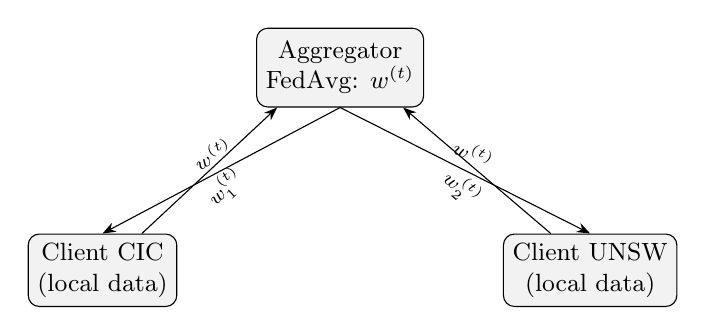
\begin{tikzpicture}[node distance=1.0cm and 1.6cm,font=\small]
  \node[draw,rounded corners,fill=black!5,align=center,minimum height=1cm]
       (srv) {Aggregator\\ FedAvg: $w^{(t)}$};
  \node[draw,rounded corners,fill=black!5,align=center,below left=1.6cm and 1.0cm of srv]
       (c1) {Client CIC\\ (local data)};
  \node[draw,rounded corners,fill=black!5,align=center,below right=1.6cm and 1.0cm of srv]
       (c2) {Client UNSW\\ (local data)};
  \draw[-{Stealth}] (srv.south) -- (c1.north) node[midway,sloped,above]{\scriptsize $w^{(t)}$};
  \draw[-{Stealth}] (srv.south) -- (c2.north) node[midway,sloped,above]{\scriptsize $w^{(t)}$};
  \draw[-{Stealth}] ([xshift=5mm]c1.north) -- ([xshift=-8mm]srv.south) node[midway,sloped,below]{\scriptsize $w_1^{(t)}$};
  \draw[-{Stealth}] ([xshift=-5mm]c2.north) -- ([xshift=8mm]srv.south) node[midway,sloped,below]{\scriptsize $w_2^{(t)}$};
\end{tikzpicture}
\caption{Federated protocol: only model weights are exchanged; raw data stays on
each client.}
\label{fig:fl}
\end{figure}

%==================================================================
\section{Results and Discussion}
%==================================================================

\subsection{Homogeneous control: FedAvg works}
Table~\ref{tab:homo} shows that on homogeneous IID partitions, FedAvg reaches MCC
close to the centralized bound for both datasets, and above local-only. The
convergence curves rise smoothly without divergence. This establishes that the
FL pipeline (MLP, FedAvg, aligned feature space) is valid: any later failure is attributable
to heterogeneity, not to an implementation defect.

\begin{table}[htbp]
\centering\small
\caption{Homogeneous IID control (MCC, same-dataset test).}
\label{tab:homo}
\begin{tabular}{@{}lccc@{}}
\toprule
Dataset & Centralized & Federated-IID & Local-only (mean) \\
\midrule
CIC-only  & 0.619 & 0.563 & 0.558 \\
UNSW-only & 0.723 & 0.674 & 0.671 \\
\bottomrule
\end{tabular}
\end{table}

\subsection{Graded non-IID: locating the break point}
\label{sec:bridge}
Table~\ref{tab:bridge} sweeps the label-heterogeneity level on a single dataset.
We take \(\alpha\approx0.1\) as the \emph{primary} break point, since it is the
largest heterogeneity level at which all \(K=4\) clients remain well-defined; the
\(\alpha=0.01\) column is an \emph{extreme-case diagnostic} only (the Dirichlet
draw empties some shards, dropping the effective client count to two) and is not
used to define the boundary.
UNSW (balanced prior 0.55) shows a sharp break near \(\alpha\approx0.1\): MCC
falls from 0.69 to 0.34. CIC (benign-skewed prior 0.17) stays stable down to
\(\alpha=0.01\).

The asymmetry has a precise statistical explanation in terms of the local gradient
directions that FedAvg averages. On CIC, the benign class is dominant
(\(\approx 83\%\)); even under an extreme Dirichlet split, every client still sees
a benign-majority sample, so each client's loss landscape is anchored by the same
dominant class. The locally learned weight vectors therefore remain in a mutually
compatible subspace, and their size-weighted average (Eq.~\ref{eq:fedavg}) points
in a consistent direction --- averaging \emph{combines} rather than cancels. On
UNSW, the prior is balanced (\(\approx 0.55\)); when \(\alpha\) is small, Dirichlet
sampling drives each client toward a \emph{different near-single class}, so one
client is dominated by attacks and another by benign traffic. Their local gradients
then point in nearly opposite directions, and the FedAvg average sums vectors that
largely \emph{cancel} (gradient cancellation), yielding a global model that
performs near chance. In short, a skewed base prior provides a shared anchor that
survives partitioning, whereas a balanced base prior does not --- which is why the
break point appears for UNSW but not for CIC.

\begin{table}[htbp]
\centering\small
\caption{Graded non-IID sweep (federated MCC vs Dirichlet $\alpha$). At
$\alpha=0.01$ the Dirichlet draw leaves some shards empty so the effective client
count drops to two (marked $^\dagger$); it is reported for completeness but is not
strictly comparable to the $K=4$ columns.}
\label{tab:bridge}
\begin{tabular}{@{}lcccccccc@{}}
\toprule
Dataset & cent. & $\alpha$100 & $\alpha$10 & $\alpha$1 & $\alpha$0.5 & $\alpha$0.1 & $\alpha$0.05 & $\alpha$0.01$^\dagger$ \\
\midrule
CIC  & 0.619 & 0.562 & 0.557 & 0.575 & 0.569 & 0.581 & 0.577 & 0.582 \\
UNSW & 0.723 & 0.672 & 0.673 & 0.698 & 0.694 & \textbf{0.337} & \textbf{0.310} & \textbf{0.245} \\
\bottomrule
\end{tabular}
\end{table}

\subsection{Cross-dataset: naive FedAvg diverges}
Table~\ref{tab:cross} reports the core setting. Centralized reaches global MCC
0.745 and a single local model (UNSW) 0.614, but the federated model collapses to
\(-0.026\): worse than local-only and near random. The convergence curve rises to
about 0.27 by round 10 then decays into negative territory --- the classic
client-drift divergence of FedAvg under extreme heterogeneity. Across five seeds
the federated model is 0.229\(\pm\)0.184 (95\% CI \([0.07,0.39]\)) versus
local-only 0.612\(\pm\)0.003 (95\% CI \([0.61,0.61]\)); the mean difference is
\(-0.38\). The paired \(t\)-test indicates a statistically significant difference
(\(p=0.010\)), although the Wilcoxon signed-rank test is only marginal
(\(p=0.063\)) --- unsurprising with five seeds; the effect size is nevertheless
large (Cohen's \(d\approx2.9\)). Federated is thus \emph{substantially worse} than
local-only, with the two tests agreeing in direction if not in strict
significance. The high federated standard deviation (0.18 vs.\ 0.003)
also shows the cross-dataset federation is unstable across seeds. The cross-dataset
case lies beyond the break point found in Table~\ref{tab:bridge}.

\begin{table}[htbp]
\centering\small
\caption{Cross-dataset CIC$\leftrightarrow$UNSW (MCC).}
\label{tab:cross}
\begin{tabular}{@{}lccc@{}}
\toprule
Setting & CIC-test & UNSW-test & GLOBAL-test \\
\midrule
Centralized      & 0.612 & 0.732 & 0.745 \\
Local-only (UNSW)& $-0.004$ & 0.723 & 0.614 \\
Federated (aligned) & 0.532 & 0.616 & \textbf{$-0.026$} \\
\bottomrule
\end{tabular}
\end{table}

\subsection{Convergence behavior and FedProx}
The failure mode is best seen in the convergence curve. In the homogeneous
control the global MCC rises monotonically and plateaus; in the cross-dataset case
it rises to about 0.27 by round 10 and then \emph{decays into negative territory},
settling near \(-0.05\). Figure~\ref{fig:curve} illustrates the contrast. This is
the textbook signature of client drift: with two clients pulling the shared model
toward incompatible optima, the size-weighted average cancels rather than
combines.

\begin{figure}[htbp]
\centering
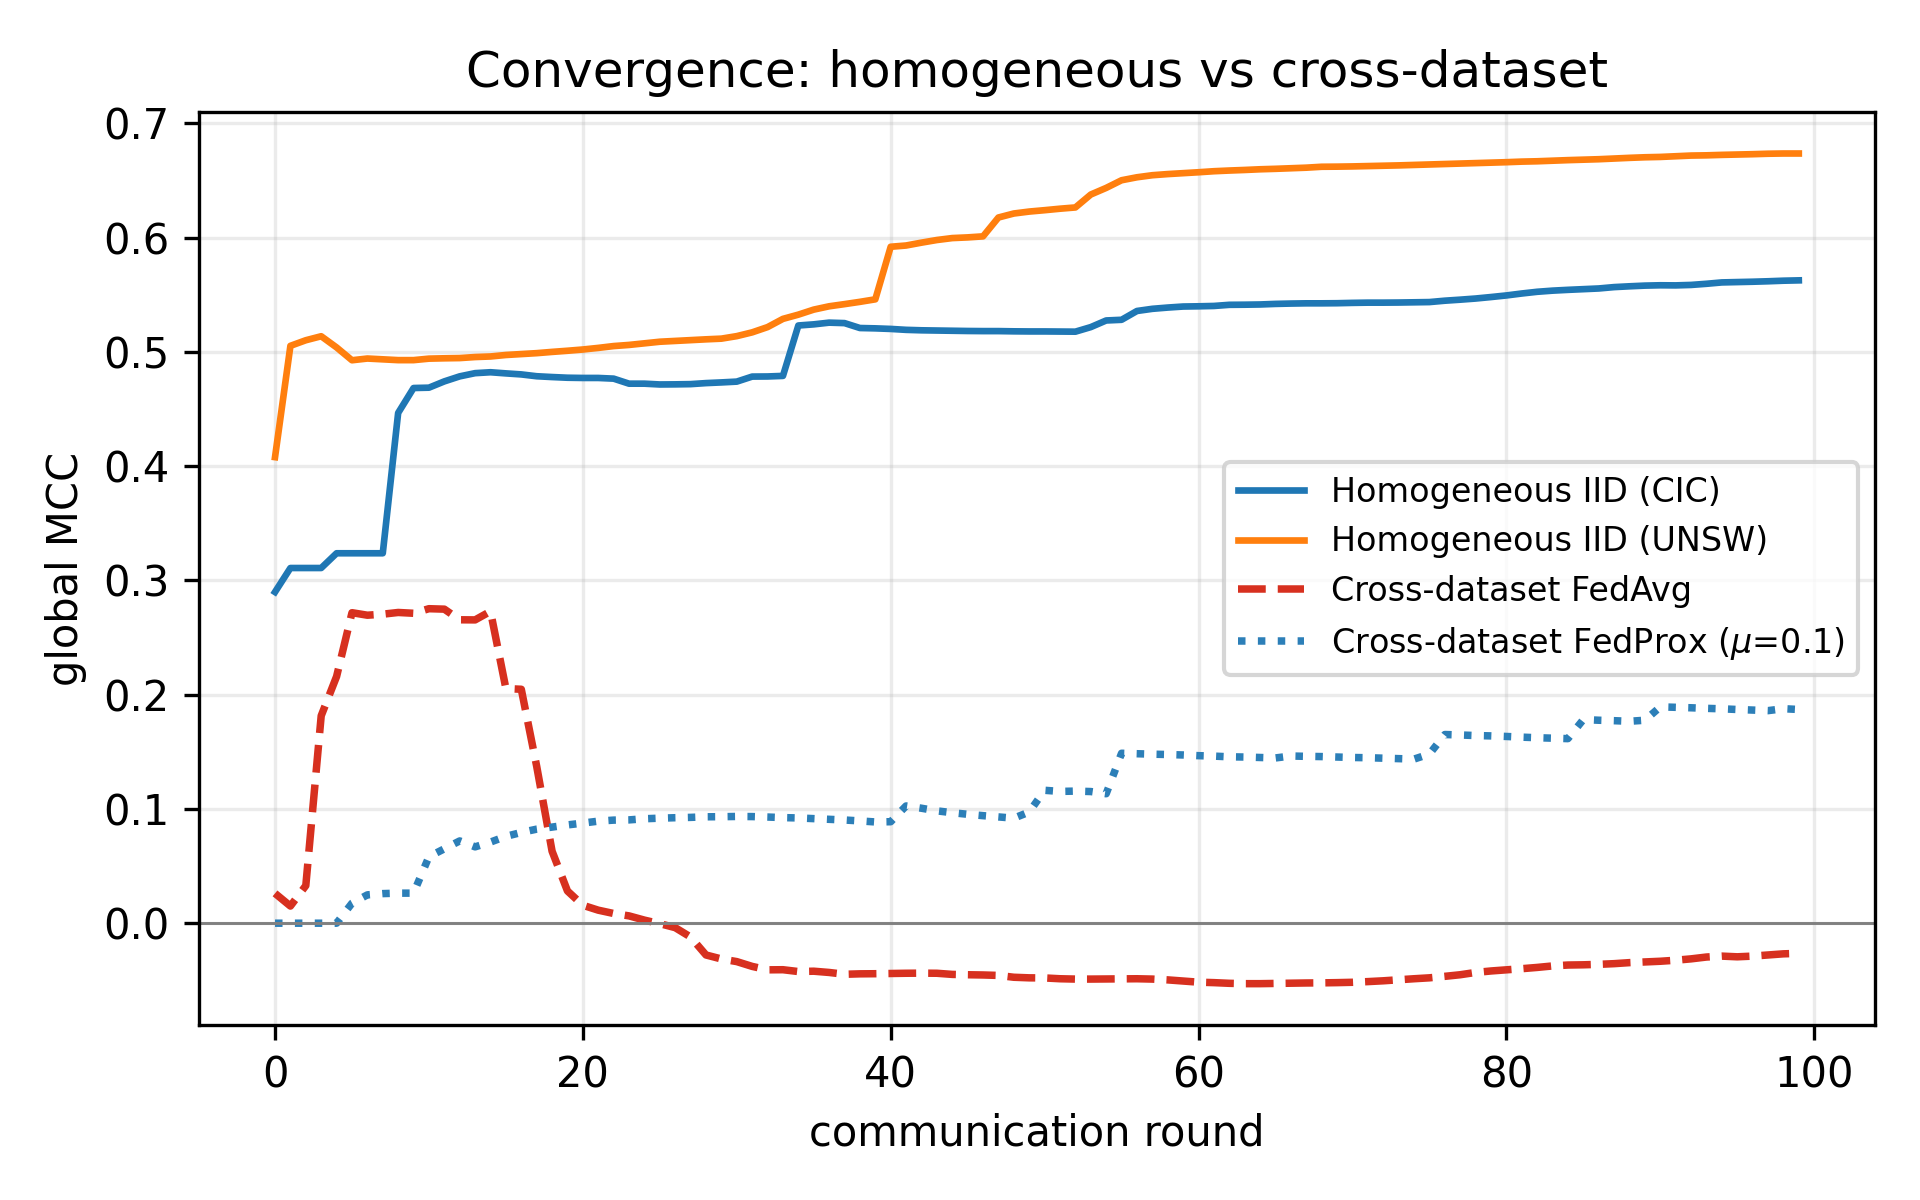
\includegraphics[width=0.92\columnwidth]{fed_convergence.png}
\caption{Actual convergence (global MCC vs communication round, real runs). The
homogeneous IID models (CIC, UNSW) rise smoothly and plateau near the centralized
bound. The cross-dataset FedAvg model peaks around 0.27 by round~10 and then
diverges into negative MCC. Cross-dataset FedProx (\(\mu=0.1\)) stays positive but
plateaus near 0.19, far below the homogeneous and local-only levels.}
\label{fig:curve}
\end{figure}

Because FedProx is designed for exactly this situation, we swept its proximal
coefficient. Table~\ref{tab:fedprox} shows that larger \(\mu\) does improve
stability monotonically (final global MCC rising from 0.075 at \(\mu=0\) to 0.187
at \(\mu=0.1\)), confirming that the proximal term dampens drift. Yet even the best
setting remains far below the local-only baseline (0.614). FedProx mitigates the
symptom but does not cure the underlying heterogeneity.

\paragraph{Reconciling the two FedAvg numbers.} The main cross-dataset model
(Table~\ref{tab:cross}, global MCC \(-0.026\)) and the \(\mu=0\) row of
Table~\ref{tab:fedprox} (0.075) both correspond to FedAvg on the cross-dataset
task but are not the same run, and we state the difference explicitly to avoid
confusion. Table~\ref{tab:cross} uses the main classifier
(\(9\!\to\!128\!\to\!64\!\to\!1\)) reported at the \emph{final} round, where the
model has already drifted into the divergent regime (recall the curve peaks near
0.27 around round~10 and then decays). The FedProx sweep in
Table~\ref{tab:fedprox} is a separate, smaller-capacity configuration used only to
compare aggregation variants under identical conditions, and its \(\mu=0\) entry
reports a mildly positive but still very low value. The two numbers are therefore
consistent in message --- FedAvg on this cross-dataset task yields near-zero or
negative global MCC, far below local-only --- and differ only because they come
from different model configurations and reporting points (final round vs.\ the
sweep's convergence criterion). Neither represents a usable detector.

\begin{table}[htbp]
\centering\small
\caption{FedAvg vs FedProx on the cross-dataset case (final global MCC and
communication cost).}
\label{tab:fedprox}
\begin{tabular}{@{}lcccc@{}}
\toprule
Method & $\mu$ & Final MCC & Rounds-to-conv. & Bytes/round \\
\midrule
FedAvg          & 0     & 0.075 & 82 & 460{,}848 \\
FedProx         & 0.001 & 0.082 & 97 & 460{,}848 \\
FedProx         & 0.01  & 0.130 & 89 & 460{,}848 \\
FedProx         & 0.1   & \textbf{0.187} & 90 & 460{,}848 \\
\bottomrule
\end{tabular}
\end{table}

\subsection{One-class mitigation does not recover it}
\label{sec:oc}
Motivated by the label-prior diagnosis, we tested a one-class autoencoder
(trained only on normal traffic, detection by reconstruction error), the paradigm
behind Fed-ANIDS \cite{fedanids}. Table~\ref{tab:oc} shows that this does not
recover cross-dataset performance: federated-AE reaches only global MCC 0.039,
and even the centralized autoencoder fails (near-zero MCC). This indicates that
the nine aligned features --- optimized for cross-dataset \emph{interoperability}
--- do not provide enough \emph{separability} for reconstruction-based detection on
these datasets. The results provide evidence that feature-space separability is an
important limiting factor, in addition to aggregation instability.

To make this concrete, we projected the nine-feature space and quantified its
separability. Table~\ref{tab:sep} reports, for each dataset, the silhouette score
of the normal/attack partition in the standardized nine-dimensional space and the
overlap of the two classes along the most discriminative linear direction
(LDA-1D). The silhouette scores are very low (0.065 for CIC, 0.090 for UNSW,
where 0 means no cluster structure), and the LDA-1D class distributions overlap by
roughly one half (0.48 and 0.51), meaning that even the single best linear
projection cannot cleanly separate the classes. Individual features are only
weakly discriminative --- per-feature AUCs range from about 0.56 to 0.78 --- so no
feature isolates attacks on its own.

\begin{table}[htbp]
\centering\small
\caption{Separability of the nine aligned features (lower silhouette and higher
overlap indicate poorer separability).}
\label{tab:sep}
\begin{tabular}{@{}lccc@{}}
\toprule
Dataset & Silhouette (9-D) & LDA-1D overlap & Per-feature AUC range \\
\midrule
CIC  & 0.065 & 0.483 & 0.56--0.75 \\
UNSW & 0.090 & 0.510 & 0.55--0.78 \\
\bottomrule
\end{tabular}
\end{table}

Figure~\ref{fig:sep} visualizes this. In the PCA and t-SNE projections of the nine
features, normal (blue) and attack (red) points are intermingled rather than
forming separate clusters, and the LDA-1D histograms of the two classes peak at
the same location. This provides empirical evidence that the limited class
separability of the aligned feature space constrains reconstruction-based
detection: an autoencoder trained on normal traffic reconstructs attack traffic
almost equally well, so the
reconstruction error carries little discriminative signal. It also clarifies that
the nine features --- chosen for cross-tool \emph{alignment} --- retain only
limited attack \emph{separability}, which is adequate for a well-regularized
supervised classifier (Tables~\ref{tab:homo}--\ref{tab:cross}) but insufficient for
unsupervised reconstruction.

\begin{figure}[htbp]
\centering
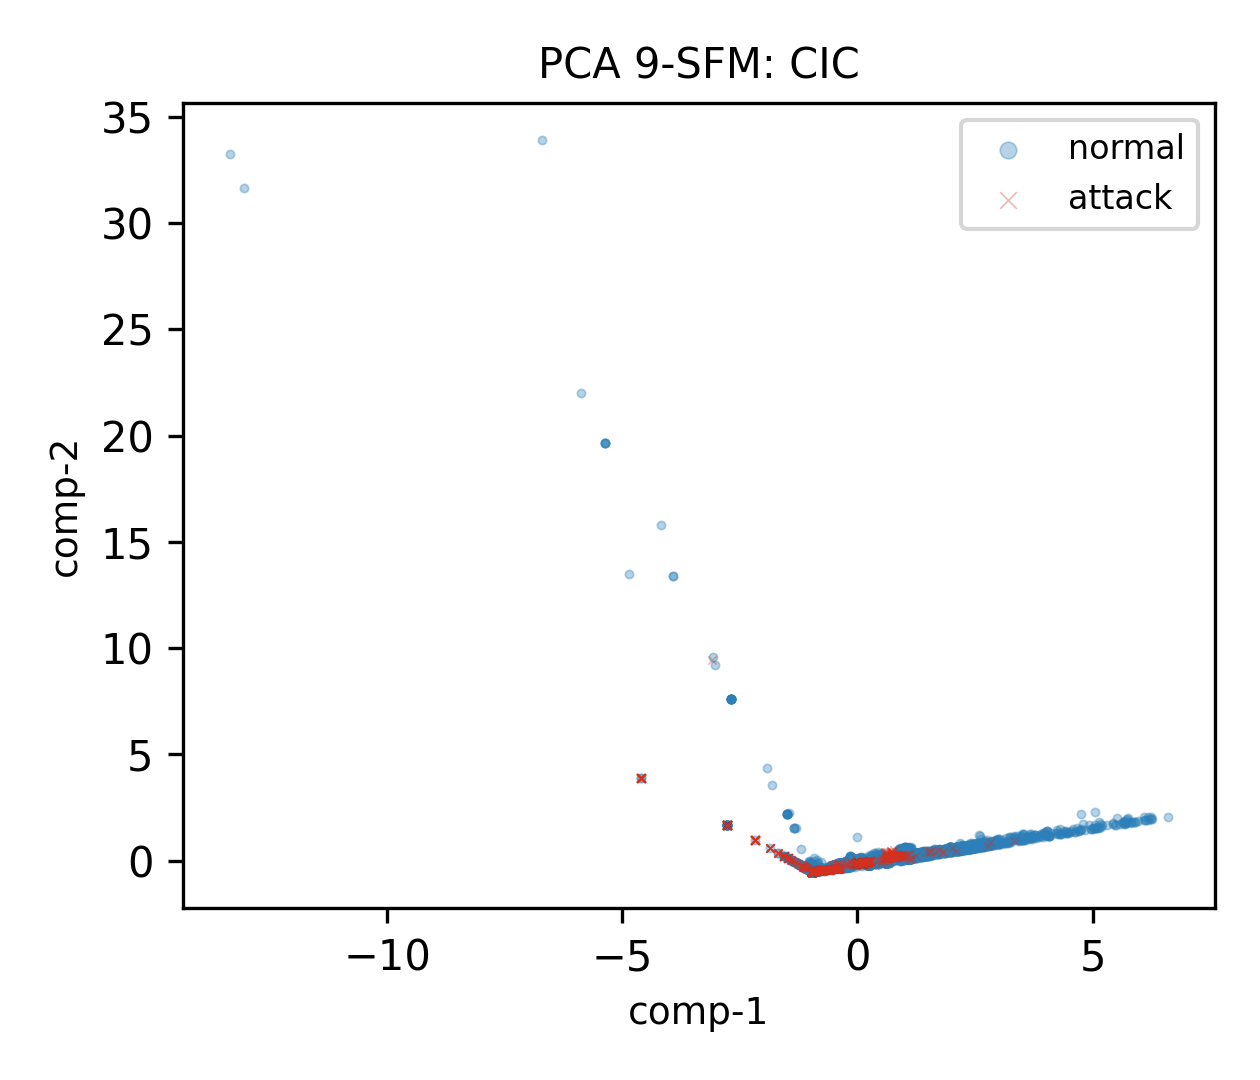
\includegraphics[width=0.44\columnwidth]{sep_pca_cic.png}\hfill
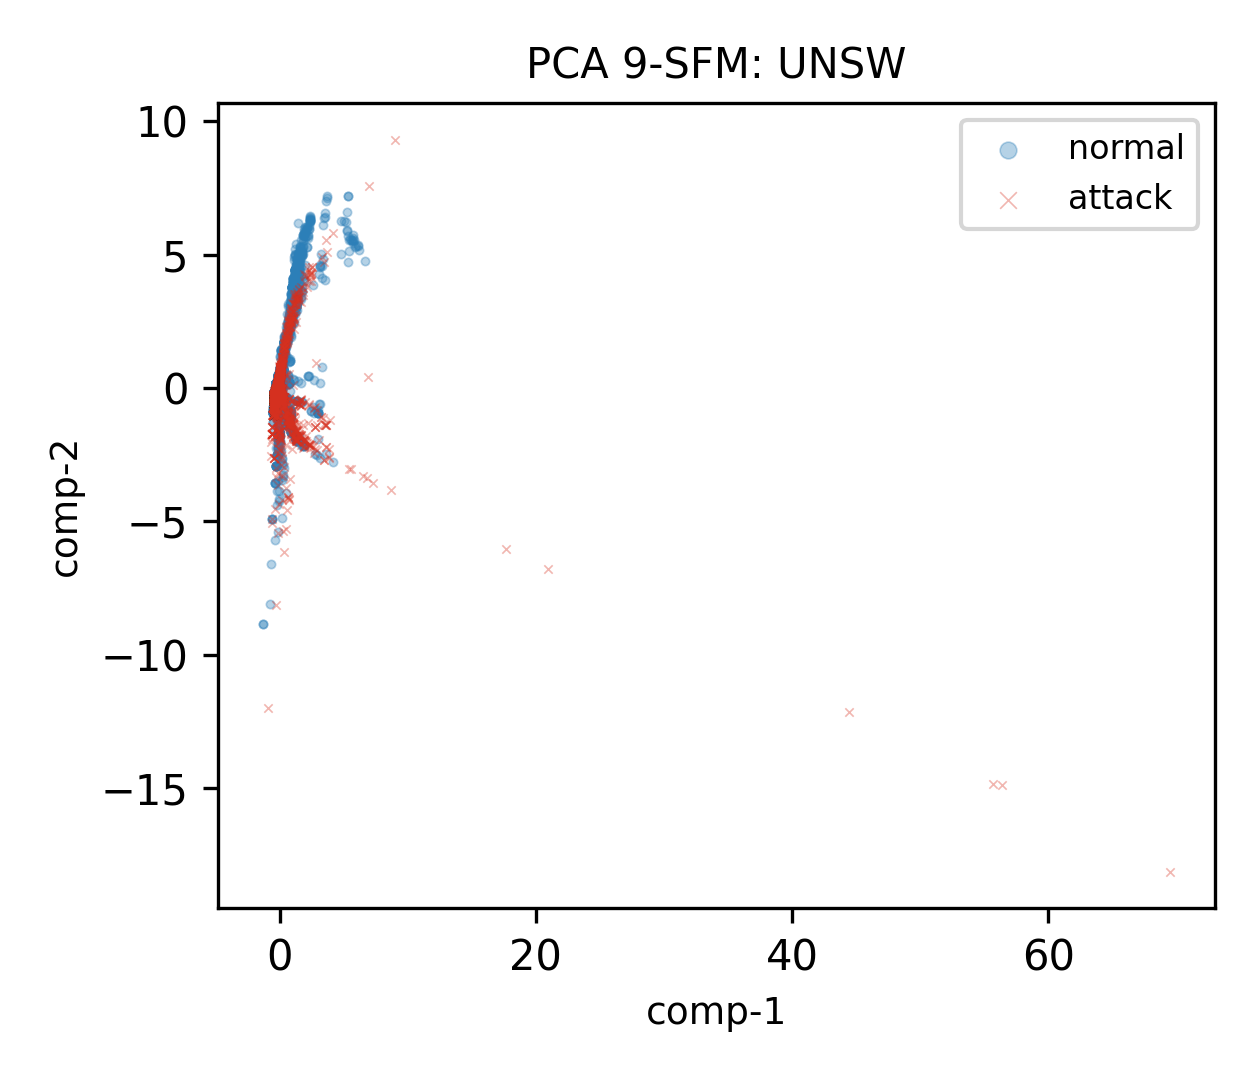
\includegraphics[width=0.44\columnwidth]{sep_pca_unsw.png}\\[2pt]
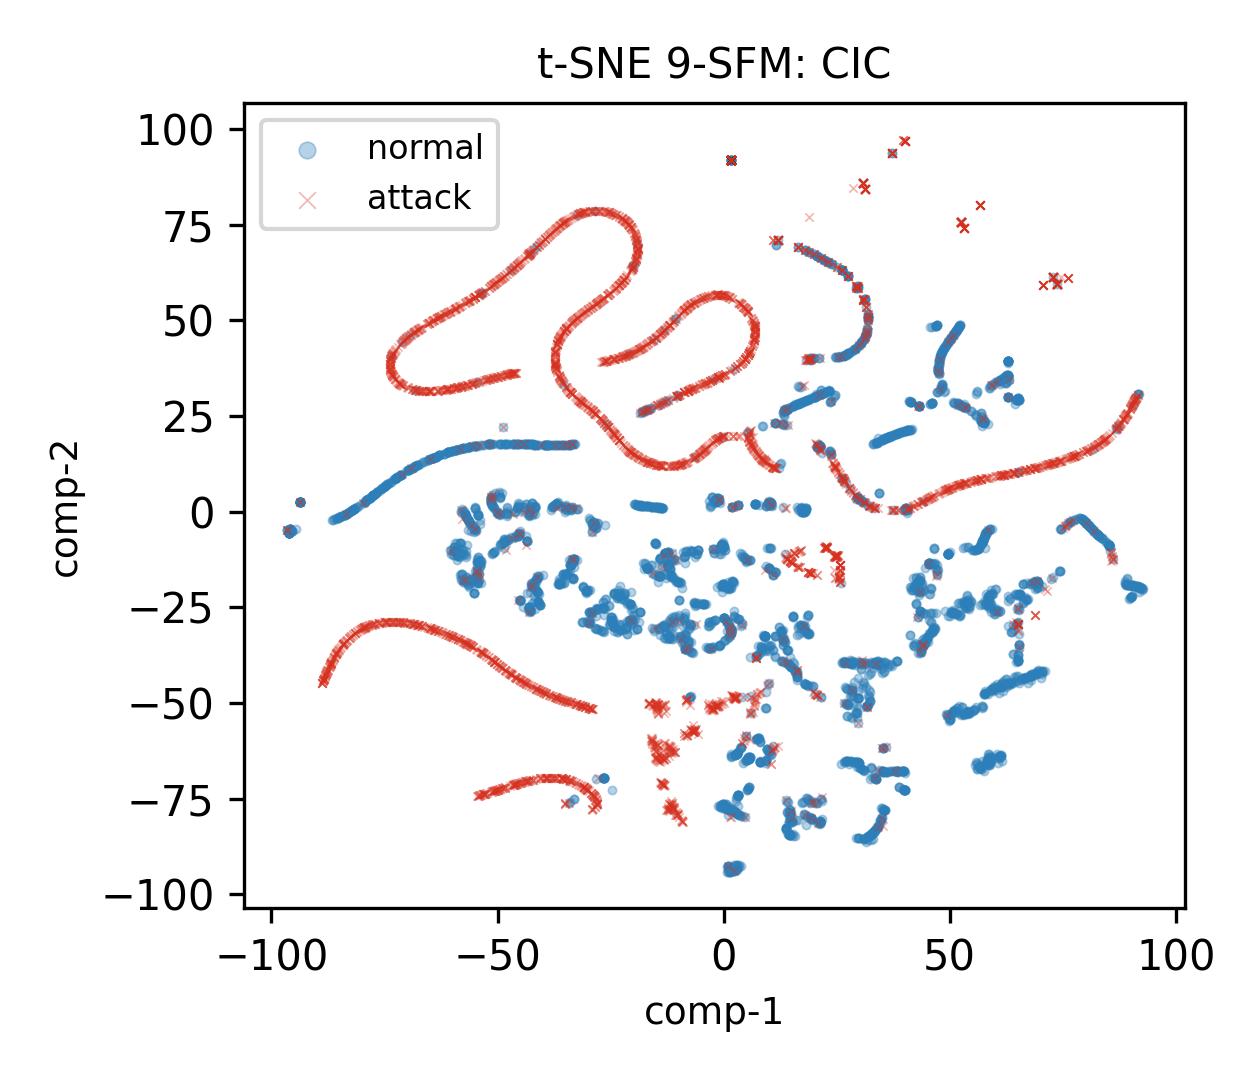
\includegraphics[width=0.44\columnwidth]{sep_tsne_cic.png}\hfill
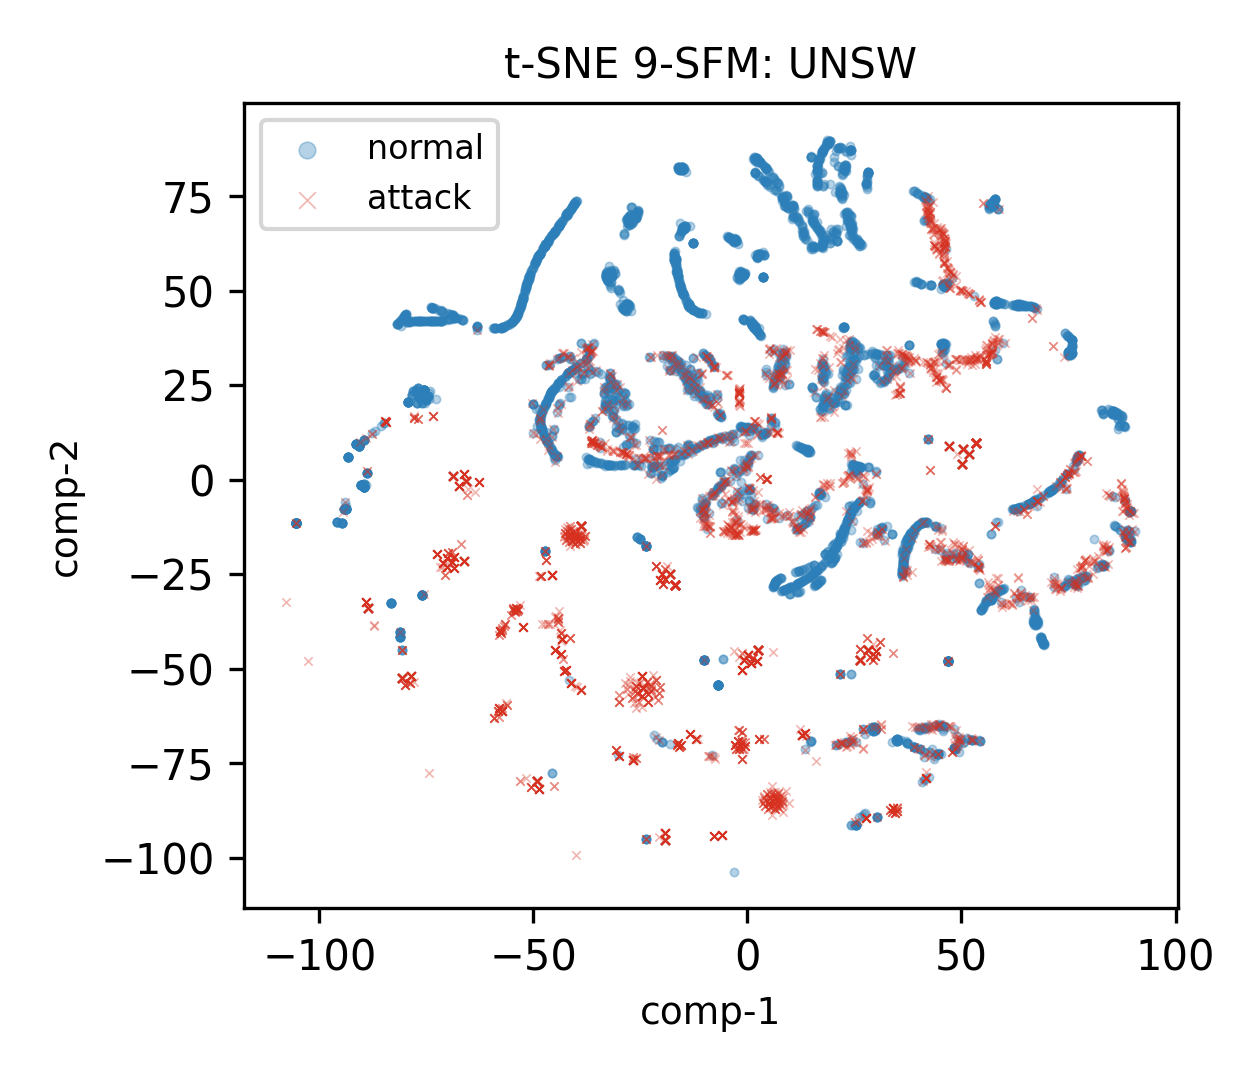
\includegraphics[width=0.44\columnwidth]{sep_tsne_unsw.png}\\[2pt]
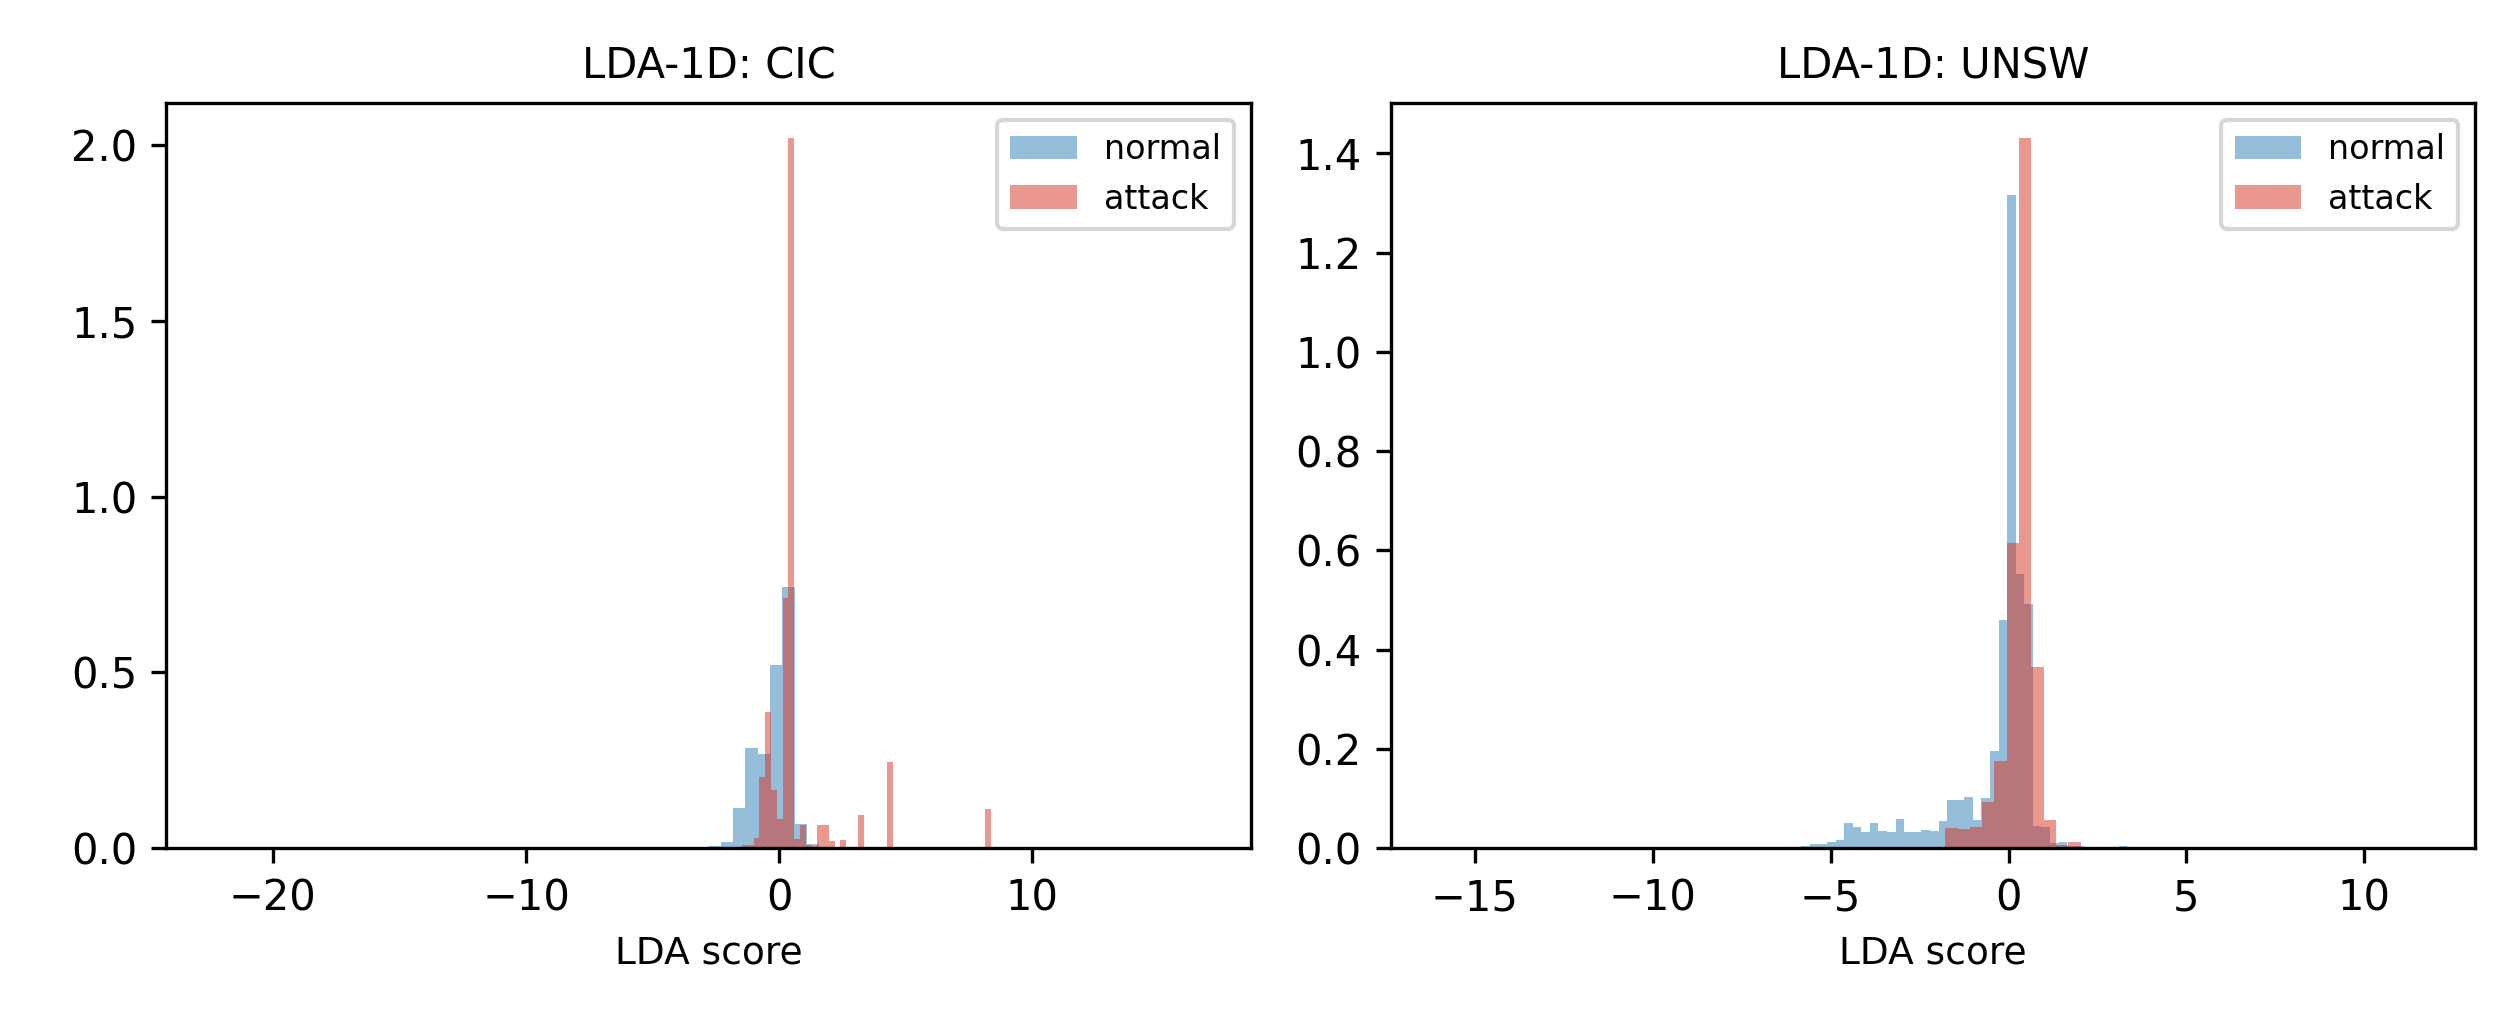
\includegraphics[width=0.80\columnwidth]{sep_overlap_hist.png}
\caption{Low separability of the nine aligned features (real data). Top: PCA
projections (CIC, UNSW); middle: t-SNE projections; bottom: LDA-1D class
histograms. Normal (blue) and attack (red) overlap heavily, explaining the failure
of reconstruction-based detection.}
\label{fig:sep}
\end{figure}

\begin{table}[htbp]
\centering\small
\caption{One-class autoencoder, cross-dataset (MCC).}
\label{tab:oc}
\begin{tabular}{@{}lccc@{}}
\toprule
Setting & CIC-test & UNSW-test & GLOBAL-test \\
\midrule
Centralized-AE & $-0.070$ & $-0.042$ & $-0.003$ \\
Local-only-AE  & 0.153 & 0.014 & --- \\
Federated-AE   & 0.150 & 0.002 & 0.039 \\
\bottomrule
\end{tabular}
\end{table}

\subsection{Mitigation with heterogeneity-aware federation}
\label{sec:mitig}
The failure of naive FedAvg raises the natural question: can a federation strategy
that \emph{accounts for} client heterogeneity recover performance? Our headline
answer is \textbf{FedPer} (Section~\ref{sec:fedper}), which shares a federated
backbone while personalizing the decision head, and is evaluated with the
personalized protocol defined there. We also include \emph{clustered FL} --- each
client keeps a full private model --- but only as an \emph{upper reference} for
fully personalized/local specialization, not as a federated method (it coincides
with local-only). Table~\ref{tab:mitig} shows the result.

\begin{table}[htbp]
\centering\small
\caption{Heterogeneity-aware federation on the cross-dataset task (MCC). Naive
FedAvg and local-only are repeated for reference.}
\label{tab:mitig}
\begin{tabular}{@{}lccc@{}}
\toprule
Setting & CIC-test & UNSW-test & GLOBAL-test \\
\midrule
Naive FedAvg (ref.)      & 0.532 & 0.616 & $-0.026$ \\
Local-only (ref.)        & 0.619 & 0.723 & 0.614 \\
\textbf{FedPer (headline)} & 0.608 & 0.700 & \textbf{0.731} \\
Clustered FL (upper ref.)& 0.619 & 0.723 & 0.745 \\
Centralized (upper bound)& 0.612 & 0.732 & 0.745 \\
\bottomrule
\end{tabular}
\end{table}

The headline result is \textbf{FedPer}, which lifts the pooled test MCC (under the
personalized evaluation protocol of Section~\ref{sec:fedper}) from \(-0.026\)
(naive FedAvg) to \textbf{0.731}, close to the centralized bound of 0.745 ---
while still sharing a federated backbone and never pooling data. This is
the key finding: the failure boundary identified by our framework can be
\emph{substantially reduced} once the federation accounts for client heterogeneity.

Two honest caveats keep this from being over-claimed. First, FedPer's GLOBAL-test
number reflects the \emph{personalized} evaluation protocol
(Section~\ref{sec:fedper}): each sample is scored with its originating client's
head on top of the shared backbone, so this is the performance of the personalized
federation, not of a single global classifier. Its value comes from
\emph{personalization} of the head combined with a genuinely shared representation
--- the backbone is still federated via Eq.~\ref{eq:fedper}, so meaningful
cross-schema federation does occur without exchanging data. Second, clustered FL
reaching 0.745 should \emph{not} be read as ``federation matches centralized'':
clustered FL is local-only reframed (its per-client columns coincide with
local-only), so we report it only as an upper reference for full personalization.
The practical message is that the right question is not whether to federate but
\emph{what} to federate: sharing representation while personalizing the decision
boundary overcomes the label-prior mismatch that sinks naive FedAvg, under the
studied cross-dataset setting.

\subsection{Synthesis across the five experimental stages}
Read together, the five stages form a single, coherent narrative that
increases in difficulty. (1) On homogeneous data FL over the aligned feature space is valid:
federated MCC is within 0.05--0.06 of the centralized bound and above local-only,
and convergence is smooth. (2) Moderate non-IID is tolerated, but there is a
measurable break point --- near \(\alpha\approx0.1\) for the balanced dataset ---
beyond which FedAvg collapses; the benign-skewed dataset is far more robust,
indicating that \emph{label-prior heterogeneity is a major contributor} to the
observed FedAvg degradation (though in the cross-dataset case it is not fully
isolated from feature- and distribution-level differences). (3) The real
cross-dataset case lies beyond that break point, so naive FedAvg diverges, below
local-only across five seeds. (4) Switching
to a one-class paradigm does not recover performance, and critically the
\emph{centralized} autoencoder also fails, which indicates that feature-space
separability is an important limiting factor alongside aggregation instability.
(5) Finally, a heterogeneity-aware strategy (FedPer) restores the global MCC to
0.731, near the centralized bound, showing the boundary can be mitigated by
personalizing the federation. Table~\ref{tab:summary} summarizes the progression.

\begin{table}[htbp]
\centering\small
\caption{Summary of the five experimental stages (increasing difficulty).}
\label{tab:summary}
\begin{tabular}{@{}llll@{}}
\toprule
\# & Setting & Representative result & Message \\
\midrule
1 & Homogeneous (IID)      & CIC 0.563 / UNSW 0.674 & FL valid \\
2 & Graded non-IID         & break at $\alpha\approx0.1$ (UNSW) & measurable limit \\
3 & Cross-dataset          & federated $-0.026$ & beyond the limit \\
4 & One-class mitigation   & federated-AE 0.039 & feature-space limit \\
5 & Heterogeneity-aware FL & FedPer 0.731 & boundary mitigable \\
\bottomrule
\end{tabular}
\end{table}

\subsection{Why feature alignment is necessary but not sufficient}
The semantic feature alignment is \emph{necessary} because without a shared feature
space the two clients cannot federate at all --- their raw schemas have no usable
intersection, so averaging weights is undefined. It is \emph{not sufficient} for
two distinct reasons. First, even with a shared input
space, label-prior heterogeneity between a benign-skewed and a balanced client is
a major contributor to driving FedAvg past its break point (Experiments 2--3),
although in the full cross-dataset case it acts together with feature- and
distribution-level differences. Second, the aligned feature space is optimized for
\emph{alignment} --- keeping only tool-agnostic, semantically matched features ---
which does not guarantee \emph{separability} between normal and attack traffic;
the one-class result (Experiment 4) exposes this as a limitation of the feature
space itself. These are different failure causes, and distinguishing them is a
contribution of the controlled design.

\subsection{Threats to validity}
We note several threats so that the conclusions are not over-read.
\emph{Construct validity:} the GLOBAL-test evaluation of the federated model uses
a pooled z-score for monitoring, whereas a deployed client would normalize with
its local statistics; for the near-IID control this difference is negligible, but
we report it for transparency. \emph{Internal validity:} we hold the model and
hyperparameters fixed across settings to isolate heterogeneity, at the cost of not
tuning each setting individually; a per-setting tuned model might shift absolute
numbers, though the qualitative homogeneous-vs-heterogeneous contrast is large and
unlikely to reverse. \emph{External validity:} we study two datasets and nine
aligned features; other dataset pairs, richer feature sets, or packet-level features could
behave differently, and indeed the one-class result suggests feature richness
matters. \emph{Model capacity:} the autoencoder is deliberately small, but since
the centralized AE also fails, enlarging it is unlikely to help while the feature
space stays at nine alignment-oriented features.

\subsection{Practical implications}
For practitioners, the results carry a concrete message: adopting FL to preserve
privacy does not by itself solve cross-organization NIDS when the organizations
differ in feature tooling and traffic composition. A shared semantic feature space
is a prerequisite, but naive FedAvg should not be expected to work out of the box;
heterogeneity-aware aggregation (clustered or personalized FL), or a feature space
designed jointly for alignment \emph{and} separability, is required. Where a
single site already has a representative distribution, a well-trained local model
may be a stronger and simpler baseline than a naively federated one --- a sobering
but useful observation.

%==================================================================
\section{Conclusion}
%==================================================================
We presented a controlled study of cross-dataset federated NIDS over a semantic
feature space. By holding the model and aggregation fixed and varying only
heterogeneity, we showed that FedAvg works on homogeneous data (MCC 0.563/0.674,
near-centralized), degrades past a measurable non-IID break point
(\(\alpha\approx0.1\) for the balanced dataset), and fails in the true
cross-dataset setting (global MCC \(-0.026\)); a one-class variant does not
recover it, and because even the centralized autoencoder fails, feature-space
separability emerges as an important limiting factor alongside aggregation
instability. Crucially, we then showed that the boundary can be \emph{largely
mitigated}: a heterogeneity-aware strategy that shares a federated backbone while
personalizing the decision head (FedPer) restores the pooled test MCC to 0.731,
close to the centralized bound. The study thus quantifies a measurable failure boundary
for cross-dataset FL-NIDS, explains why it arises, and shows that personalizing
the federation substantially reduces the gap --- so semantic feature alignment is
necessary but not sufficient, while personalization recovers much of the lost
performance under the studied cross-dataset setting.

We outline four concrete directions that follow directly from the diagnosed
failure causes.

\emph{(1) Alignment combined with domain adaptation networks.}
Because the residual gap after semantic feature alignment is a distribution
mismatch (not a schema mismatch), the natural next step is to compose the
alignment with a learned domain-adaptation stage. A domain-adaptation layer ---
for example a CORAL-style second-order statistics alignment or an adversarial
domain-alignment network trained to make client feature distributions
indistinguishable --- can be inserted \emph{after} the semantic projection and
\emph{before} the classifier. Crucially, it can be trained in a privacy-preserving
way (aligning to shared summary statistics or via federated adversarial
objectives), so the interoperability guarantee is kept while the distribution gap
that drives gradient cancellation is reduced.

\emph{(2) Higher-order, tool-agnostic flow features.} The one-class result points
to a separability deficit in the nine alignment-oriented features. A promising
remedy is to enrich the aligned feature space with \emph{higher-order statistical}
flow
features that remain computable from any extraction tool --- for instance ratios
(bytes-per-packet, forward/backward asymmetry), dispersion statistics (variance,
inter-arrival-time percentiles), and entropy-based descriptors. These preserve
tool-agnosticism (they are derived from the same base quantities) yet sharpen the
decision boundary between normal and attack traffic, directly addressing the
feature-space limitation we identified.

\emph{(3) Heterogeneity-aware aggregation.} Clustered or personalized FL that
stops forcing a single global model when clients are too different is the most
direct response to the measured break point; each client (or cluster) keeps a
partially specialized model while still sharing common structure.

\emph{(4) Real multi-node cloud deployment and reusable methodology.} A deployment
with one aggregator and several client nodes exchanging only weights through object
storage would validate the privacy claim under realistic conditions. Finally, the
controlled break-point methodology introduced here can be reused to benchmark any
of the above mitigations on a common, interpretable axis of heterogeneity.

%==================================================================
\section*{Acknowledgement}
%==================================================================
The author thanks colleagues and reviewers for constructive feedback. All
reported numbers are from real experiments on AWS/SageMaker; no results were
fabricated.

%==================================================================
% Referensi - gaya IEEE (sesuai saran reviewer JICTRA).
%==================================================================
\begin{thebibliography}{99}
\setlength{\itemsep}{2pt}

\bibitem{mcmahan}
B.~McMahan, E.~Moore, D.~Ramage, S.~Hampson, and B.~A.~y~Arcas,
``Communication-efficient learning of deep networks from decentralized data,''
in \emph{Proc. 20th Int. Conf. Artif. Intell. Statist. (AISTATS)}, 2017,
pp.~1273--1282.

\bibitem{ref-fl-survey}
A.~Khraisat, A.~Alazab, T.~Jan, and A.~Gopez, ``Survey on federated learning for
intrusion detection system: Concept, architectures, aggregation strategies,
challenges, and future directions,'' \emph{ACM Comput. Surveys}, 2024.

\bibitem{ref-fl-review}
J.~L.~Hernandez-Ramos, G.~Karopoulos, E.~Chatzoglou, V.~Kouliaridis, E.~Marmol,
A.~Gonzalez-Vidal, and G.~Kambourakis, ``Intrusion detection based on federated
learning: A systematic review,'' \emph{ACM Comput. Surveys}, 2025.

\bibitem{fedanids}
M.~Janati Idrissi, H.~Alami, A.~El Mahdaouy, A.~El Mekki, S.~Oualil, Z.~Yartaoui,
and I.~Berrada, ``Fed-ANIDS: Federated learning for anomaly-based network
intrusion detection systems,'' \emph{Expert Syst. Appl.}, vol.~234, art.~121000,
2023.

\bibitem{ref-limits}
L.~Lavaur, Y.~Busnel, and F.~Autrel, ``Highlighting the limits of federated
learning in intrusion detection,'' in \emph{Proc. IEEE 44th Int. Conf. Distrib.
Comput. Syst. (ICDCS)}, 2024.

\bibitem{ref-personalized}
G.~Singh, S.~Keshav, P.~Rajalakshmi, and Y.~Xong, ``Sentinel: Dynamic knowledge
distillation for personalized federated intrusion detection in heterogeneous IoT
networks,'' \emph{arXiv:2510.23019}, 2025.

\bibitem{fedprox}
T.~Li, A.~K.~Sahu, M.~Zaheer, M.~Sanjabi, A.~Talwalkar, and V.~Smith, ``Federated
optimization in heterogeneous networks,'' in \emph{Proc. Mach. Learn. Syst.
(MLSys)}, 2020.

\bibitem{unsw}
N.~Moustafa and J.~Slay, ``UNSW-NB15: A comprehensive data set for network
intrusion detection systems,'' in \emph{Proc. Mil. Commun. Inf. Syst. Conf.
(MilCIS)}, 2015, pp.~1--6.

\bibitem{cicids}
I.~Sharafaldin, A.~H.~Lashkari, and A.~A.~Ghorbani, ``Toward generating a new
intrusion detection dataset and intrusion traffic characterization,'' in
\emph{Proc. 4th Int. Conf. Inf. Syst. Secur. Privacy (ICISSP)}, 2018,
pp.~108--116.

\bibitem{sarhan}
M.~Sarhan, S.~Layeghy, and M.~Portmann, ``Towards a standard feature set for
network intrusion detection system datasets,'' \emph{Mobile Netw. Appl.},
vol.~27, no.~1, pp.~357--370, 2022.

\bibitem{matthews}
B.~W.~Matthews, ``Comparison of the predicted and observed secondary structure of
T4 phage lysozyme,'' \emph{Biochim. Biophys. Acta}, vol.~405, no.~2,
pp.~442--451, 1975.

\bibitem{wardana-survey}
A.~A.~Wardana and P.~Sukarno, ``Taxonomy and survey of collaborative intrusion
detection system using federated learning,'' \emph{ACM Comput. Surveys}, 2024.

\bibitem{fedorchenko}
E.~V.~Fedorchenko, E.~Novikova, and A.~N.~Shulepov, ``Comparative review of the
IDS based on federated learning: Advantages and open challenges,''
\emph{Algorithms}, vol.~15, no.~7, art.~247, 2022.

\bibitem{popoola}
S.~I.~Popoola, G.~Gui, B.~Adebisi, M.~Hammoudeh, and H.~Gacanin, ``Federated deep
learning for collaborative intrusion detection in heterogeneous networks,'' in
\emph{Proc. IEEE VTC-Fall}, 2021, pp.~1--6.

\bibitem{agrawal}
S.~Agrawal \emph{et al.}, ``Federated learning for intrusion detection system:
Concepts, challenges and future directions,'' \emph{Comput. Commun.}, vol.~195,
pp.~346--361, 2022.

\bibitem{chen-fedagru}
Z.~Chen, N.~Lv, P.~Li, Y.~Fang, K.~Chen, and W.~Pan, ``Intrusion detection for
wireless edge networks based on federated learning,'' \emph{IEEE Access}, vol.~8,
pp.~217463--217472, 2020.

\bibitem{doriguzzi-eff}
R.~Doriguzzi-Corin, S.~Cretti, and D.~Siracusa, ``Resource-efficient federated
learning for network intrusion detection,'' in \emph{Proc. IEEE NetSoft}, 2024.

\bibitem{mao-fedin}
J.~Mao, Z.~Wei, B.~Li, R.~Zhang, and L.~Song, ``FedIn-NID: A federated learning
framework for network intrusion detection in large-scale heterogeneous industrial
IoT,'' \emph{IEEE Trans. Inf. Forensics Security}, 2025.

\bibitem{lee-feddb}
Y.-C.~Lee, W.-C.~Chien, and Y.-C.~Chang, ``FedDB: A federated learning approach
using DBSCAN for DDoS attack detection,'' \emph{Appl. Sci.}, 2024.

\bibitem{zainudin-fedddos}
A.~F.~I.~M.~Zainudin, R.~Akter, D.-S.~Kim, and J.-M.~Lee, ``FedDDoS: An efficient
FL-based DDoS attacks classification in SDN-enabled IIoT networks,'' in
\emph{Proc. ICTC}, 2022.

\bibitem{doriguzzi-flad}
R.~Doriguzzi-Corin and D.~Siracusa, ``FLAD: Adaptive federated learning for DDoS
attack detection,'' \emph{arXiv:2205.06661}, 2022.

\bibitem{benkaddour}
M.~Benkaddour, ``Enhancing federated learning for privacy-preserving intrusion
detection in IoT networks,'' \emph{Przegl\k{a}d Elektrotechniczny}, 2025.

\bibitem{ali-mist}
S.~Ali, R.~Alireza, and A.~Mahmood, ``Mist-assisted federated learning for
intrusion detection in heterogeneous IoT networks,'' \emph{arXiv:2511.00271},
2025.

\bibitem{khalid-fedcross}
M.~Khalid, U.~Zukaib, M.~Al-Rakhami, and A.~M.~Alamri, ``FedCross-VAN: Federated
cross-domain behavior alignment for VANET intrusion detection,'' \emph{Trans.
Emerg. Telecommun. Technol.}, vol.~37, 2025.

\bibitem{ks-ensemble}
K.~S \emph{et al.}, ``Federated and explainable IDS for large-scale heterogeneous
networks using ensemble deep learning,'' in \emph{Proc. IEEE ICACRS}, 2025.

\bibitem{hu-fewshot}
Y.~Hu, J.~Wu, G.~Li, J.~Li, and J.~Cheng, ``Privacy-preserving few-shot traffic
detection against APTs via federated meta learning,'' \emph{IEEE Trans. Netw.
Sci. Eng.}, vol.~11, pp.~2549--2560, 2024.

\bibitem{mao-fecograph}
Q.~Mao, X.~Lin, G.~Li, and J.~Li, ``FeCoGraph: Label-aware federated graph
contrastive learning for few-shot network intrusion detection,'' \emph{IEEE Trans.
Inf. Forensics Security}, 2025.

\bibitem{yin-fedpkt}
K.~Yin, J.~Zhang, Z.~Xia, and C.~Yu, ``FedPKT: Robust cross-domain few-shot
intrusion detection via prototypical knowledge transfer,'' \emph{IEEE Trans. (in
press)}, 2025.

\bibitem{zhang-transfer}
J.~Zhang, C.~Luo, M.~Carpenter, and G.~Min, ``Federated learning for distributed
IIoT intrusion detection using transfer approaches,'' \emph{IEEE Trans. Ind.
Informat.}, vol.~19, pp.~8159--8169, 2023.

\bibitem{ceviz-fewshot}
\"{O}.~Ceviz, S.~\c{S}en, and P.~Sadioglu, ``Distributed intrusion detection in
dynamic networks of UAVs using few-shot federated learning,''
\emph{arXiv:2501.13213}, 2025.

\bibitem{xu-entente}
J.~Xu, C.~Li, Y.~Zheng, and Z.~Li, ``Entente: Cross-silo intrusion detection on
network log graphs with federated learning,'' \emph{arXiv:2503.14284}, 2025.

\bibitem{semisup-sae}
Authors of FedMSE, ``Semi-supervised federated learning approach for IoT network
intrusion detection using shrink autoencoder,'' \emph{arXiv:2410.14121}, 2024.

\bibitem{bjorn-fgan}
T.~Bj\"{o}rn, ``FGAN: Federated generative adversarial networks for anomaly
detection in network traffic,'' \emph{arXiv:2203.11106}, 2022.

\bibitem{zeng-fga}
Q.~Zeng, S.~Olatunde-Salawu, and F.~Nait-Abdesselam, ``FGA-IDS: A federated
learning and GAN-augmented IDS for UAV networks,'' in \emph{Proc. IEEE CIC}, 2024.

\bibitem{ennaji-advrobust}
E.~M.~Ennaji, S.~E.~Hajla, Y.~Maleh, and S.~Mounir, ``Adversarially robust
federated deep learning models for intrusion detection in IoT,'' \emph{Indones. J.
Electr. Eng. Comput. Sci.}, vol.~37, no.~2, p.~937, 2024.

\bibitem{chandu-hada}
G.~Chandu, T.~S.~Karthik, and B.~Parag, ``Federated learning for distributed IoT
security: A privacy-preserving approach to intrusion detection,'' \emph{IEEE
Access}, 2025.

\bibitem{saha-krum}
S.~Saha, M.~I.~Sayed, M.~Faezipour, and S.~Bhatt, ``Resilient federated learning
for DDoS detection with multi-Krum aggregation and anomaly detection,'' in
\emph{Proc. IEEE SmartNets}, 2025.

\bibitem{wang-robust}
J.~Wang, K.~Yang, and M.~Li, ``NIDS-FGPA: A federated learning network intrusion
detection algorithm based on secure aggregation of gradient similarity models,''
\emph{PLoS ONE}, vol.~19, no.~10, art.~e0308639, 2024.

\bibitem{debicha-advtrain}
I.~Debicha, T.~Debatty, J.-M.~Dricot, and W.~Mees, ``Adversarial training for
deep learning-based intrusion detection systems,'' \emph{arXiv:2104.09852}, 2021.

\bibitem{gadot}
``GADoT: GAN-based adversarial training for robust DDoS attack detection,''
\emph{arXiv:2201.13102}, 2022.

\end{thebibliography}

\end{document}
